\documentclass{standalone}
\usepackage{tikz}
\usetikzlibrary{patterns, positioning}
\usepackage[sfdefault]{ClearSans} %% option 'sfdefault' activates Clear Sans as the default text font
\usepackage[T1]{fontenc}

\begin{document}
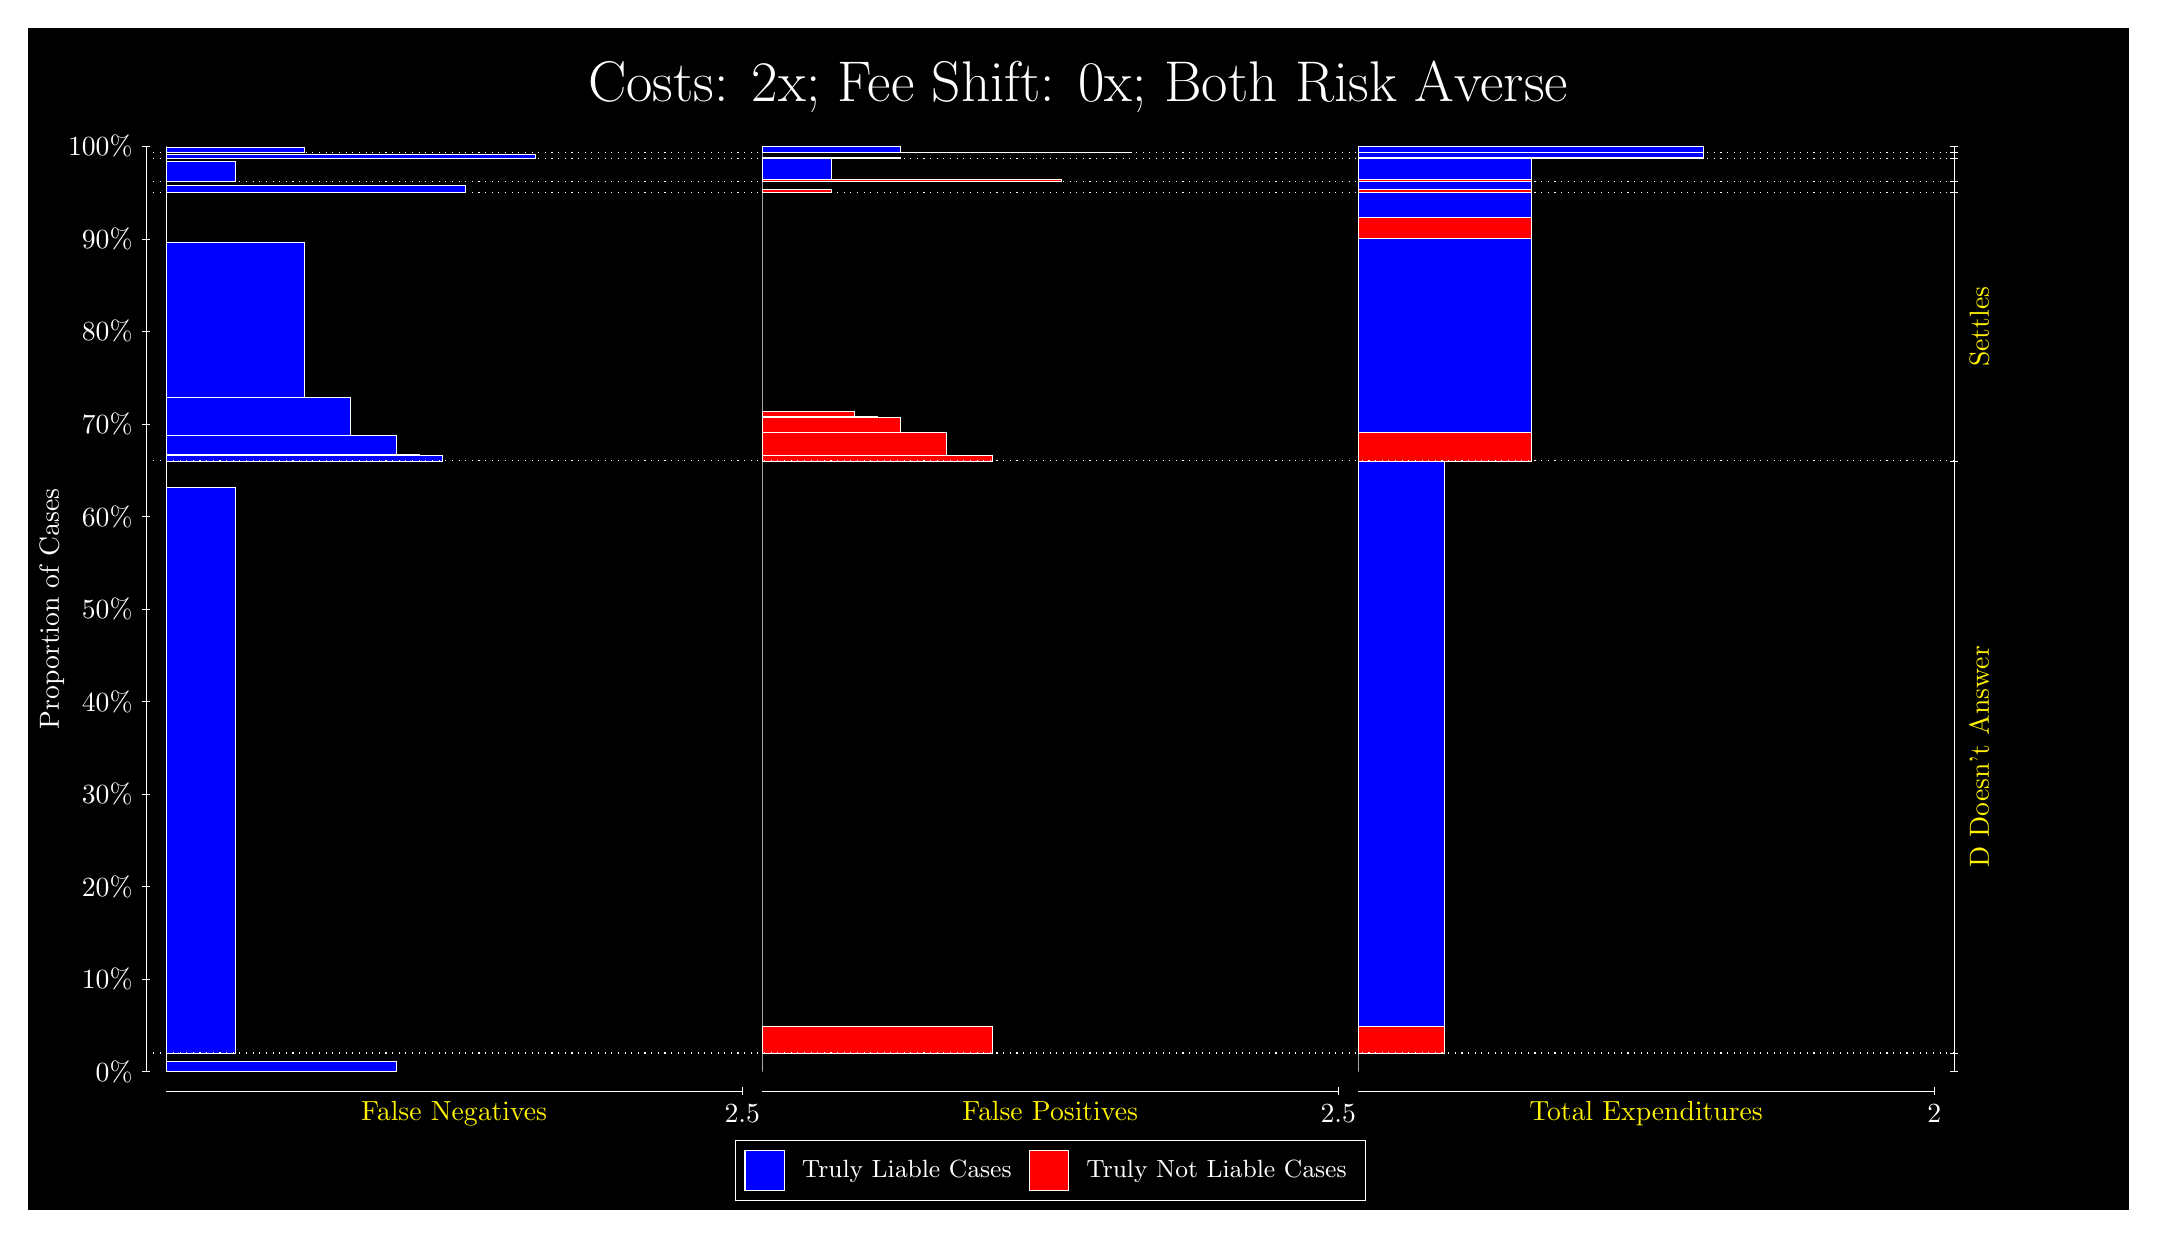
\begin{tikzpicture}
\draw[fill=black] (0,0) rectangle (26.667,15);
\draw[text=white] (0,13.5) rectangle (26.667,15) node[midway] {\huge Costs: 2x; Fee Shift: 0x; Both Risk Averse};
\draw[white, very thin] (1.5,1.75) -- (1.5,13.5);
\node[rotate=90, text=white, anchor=center] at (0.3, 7.625) {Proportion of Cases};
\draw[white, very thin] (1.45,1.75) -- (1.55,1.75);
\node[text=white, anchor=east] at (1.45, 1.75) {0\%};
\draw[white, very thin] (1.45,2.925) -- (1.55,2.925);
\node[text=white, anchor=east] at (1.45, 2.925) {10\%};
\draw[white, very thin] (1.45,4.1) -- (1.55,4.1);
\node[text=white, anchor=east] at (1.45, 4.1) {20\%};
\draw[white, very thin] (1.45,5.275) -- (1.55,5.275);
\node[text=white, anchor=east] at (1.45, 5.275) {30\%};
\draw[white, very thin] (1.45,6.45) -- (1.55,6.45);
\node[text=white, anchor=east] at (1.45, 6.45) {40\%};
\draw[white, very thin] (1.45,7.625) -- (1.55,7.625);
\node[text=white, anchor=east] at (1.45, 7.625) {50\%};
\draw[white, very thin] (1.45,8.8) -- (1.55,8.8);
\node[text=white, anchor=east] at (1.45, 8.8) {60\%};
\draw[white, very thin] (1.45,9.975) -- (1.55,9.975);
\node[text=white, anchor=east] at (1.45, 9.975) {70\%};
\draw[white, very thin] (1.45,11.15) -- (1.55,11.15);
\node[text=white, anchor=east] at (1.45, 11.15) {80\%};
\draw[white, very thin] (1.45,12.325) -- (1.55,12.325);
\node[text=white, anchor=east] at (1.45, 12.325) {90\%};
\draw[white, very thin] (1.45,13.5) -- (1.55,13.5);
\node[text=white, anchor=east] at (1.45, 13.5) {100\%};

\draw[white, very thin] (24.457,1.75) -- (24.457,13.5);
\draw[white, very thin] (24.407,1.75) -- (24.507,1.75);
\node[anchor=west] at (24.407, 1.75) {};
\draw[white, very thin] (24.407,1.9847) -- (24.507,1.9847);
\node[anchor=west] at (24.407, 1.9847) {};
\draw[white, very thin] (24.407,9.5064) -- (24.507,9.5064);
\node[anchor=west] at (24.407, 9.5064) {};
\draw[white, very thin] (24.407,12.913) -- (24.507,12.913);
\node[anchor=west] at (24.407, 12.913) {};
\draw[white, very thin] (24.407,13.056) -- (24.507,13.056);
\node[anchor=west] at (24.407, 13.056) {};
\draw[white, very thin] (24.407,13.343) -- (24.507,13.343);
\node[anchor=west] at (24.407, 13.343) {};
\draw[white, very thin] (24.407,13.423) -- (24.507,13.423);
\node[anchor=west] at (24.407, 13.423) {};
\draw[white, very thin] (24.407,13.5) -- (24.507,13.5);
\node[anchor=west] at (24.407, 13.5) {};

\draw[white, very thin, fill=blue] (1.75,1.75) rectangle (4.6775,1.8827);
\draw[white, very thin, fill=red] (1.75,1.8827) rectangle (1.75,1.9847);
\draw[white, very thin, fill=blue] (1.75,1.9847) rectangle (2.6283,9.1652);
\draw[white, very thin, fill=red] (1.75,9.1652) rectangle (1.75,9.5064);
\draw[white, very thin, fill=blue] (1.75,9.5064) rectangle (5.2631,9.5774);
\draw[white, very thin, fill=blue] (1.75,9.5774) rectangle (4.9703,9.5868);
\draw[white, very thin, fill=blue] (1.75,9.5868) rectangle (4.6775,9.8254);
\draw[white, very thin, fill=blue] (1.75,9.8254) rectangle (4.092,10.313);
\draw[white, very thin, fill=blue] (1.75,10.313) rectangle (3.5065,12.284);
\draw[white, very thin, fill=red] (1.75,12.284) rectangle (1.75,12.913);
\draw[white, very thin, fill=blue] (1.75,12.913) rectangle (5.5558,13.011);
\draw[white, very thin, fill=red] (1.75,13.011) rectangle (1.75,13.056);
\draw[white, very thin, fill=blue] (1.75,13.056) rectangle (2.6283,13.313);
\draw[white, very thin, fill=red] (1.75,13.313) rectangle (1.75,13.343);
\draw[white, very thin, fill=blue] (1.75,13.343) rectangle (6.4341,13.402);
\draw[white, very thin, fill=red] (1.75,13.402) rectangle (1.75,13.423);
\draw[white, very thin, fill=blue] (1.75,13.423) rectangle (3.5065,13.493);
\draw[white, very thin, fill=red] (1.75,13.493) rectangle (1.75,13.5);
\draw[white, very thin, fill=red] (9.3189,1.75) rectangle (9.3189,1.852);
\draw[white, very thin, fill=blue] (9.3189,1.852) rectangle (9.3189,1.9847);
\draw[white, very thin, fill=red] (9.3189,1.9847) rectangle (12.246,2.3259);
\draw[white, very thin, fill=blue] (9.3189,2.3259) rectangle (9.3189,9.5064);
\draw[white, very thin, fill=red] (9.3189,9.5064) rectangle (12.246,9.5786);
\draw[white, very thin, fill=red] (9.3189,9.5786) rectangle (11.661,9.868);
\draw[white, very thin, fill=red] (9.3189,9.868) rectangle (11.075,10.063);
\draw[white, very thin, fill=red] (9.3189,10.063) rectangle (10.783,10.069);
\draw[white, very thin, fill=red] (9.3189,10.069) rectangle (10.49,10.135);
\draw[white, very thin, fill=blue] (9.3189,10.135) rectangle (9.3189,12.913);
\draw[white, very thin, fill=red] (9.3189,12.913) rectangle (10.197,12.958);
\draw[white, very thin, fill=blue] (9.3189,12.958) rectangle (9.3189,13.056);
\draw[white, very thin, fill=red] (9.3189,13.056) rectangle (13.125,13.086);
\draw[white, very thin, fill=blue] (9.3189,13.086) rectangle (10.197,13.343);
\draw[white, very thin, fill=red] (9.3189,13.343) rectangle (11.075,13.364);
\draw[white, very thin, fill=blue] (9.3189,13.364) rectangle (9.3189,13.423);
\draw[white, very thin, fill=red] (9.3189,13.423) rectangle (14.003,13.43);
\draw[white, very thin, fill=blue] (9.3189,13.43) rectangle (11.075,13.5);
\draw[white, very thin, fill=red] (16.888,1.75) rectangle (16.888,1.852);
\draw[white, very thin, fill=blue] (16.888,1.852) rectangle (16.888,1.9847);
\draw[white, very thin, fill=red] (16.888,1.9847) rectangle (17.986,2.3259);
\draw[white, very thin, fill=blue] (16.888,2.3259) rectangle (17.986,9.5064);
\draw[white, very thin, fill=red] (16.888,9.5064) rectangle (19.083,9.868);
\draw[white, very thin, fill=blue] (16.888,9.868) rectangle (19.083,12.327);
\draw[white, very thin, fill=red] (16.888,12.327) rectangle (19.083,12.594);
\draw[white, very thin, fill=blue] (16.888,12.594) rectangle (19.083,12.913);
\draw[white, very thin, fill=red] (16.888,12.913) rectangle (19.083,12.958);
\draw[white, very thin, fill=blue] (16.888,12.958) rectangle (19.083,13.056);
\draw[white, very thin, fill=red] (16.888,13.056) rectangle (19.083,13.086);
\draw[white, very thin, fill=blue] (16.888,13.086) rectangle (19.083,13.343);
\draw[white, very thin, fill=red] (16.888,13.343) rectangle (21.279,13.364);
\draw[white, very thin, fill=blue] (16.888,13.364) rectangle (21.279,13.423);
\draw[white, very thin, fill=red] (16.888,13.423) rectangle (21.279,13.43);
\draw[white, very thin, fill=blue] (16.888,13.43) rectangle (21.279,13.5);
\draw[white, dotted] (1.5,1.9847) -- (24.457,1.9847);
\draw[white, dotted] (1.5,9.5064) -- (24.457,9.5064);
\draw[white, dotted] (1.5,12.913) -- (24.457,12.913);
\draw[white, dotted] (1.5,13.056) -- (24.457,13.056);
\draw[white, dotted] (1.5,13.343) -- (24.457,13.343);
\draw[white, dotted] (1.5,13.423) -- (24.457,13.423);
\draw[white, very thin] (1.75,1.5) -- (9.0689,1.5);
\node[text=yellow, anchor=north] at (5.4094, 1.5) {False Negatives};
\draw[white, very thin] (9.0689,1.45) -- (9.0689,1.55);
\node[text=white, anchor=north] at (9.0689, 1.45) {2.5};

\draw[white, very thin] (9.3189,1.5) -- (16.638,1.5);
\node[text=yellow, anchor=north] at (12.978, 1.5) {False Positives};
\draw[white, very thin] (16.638,1.45) -- (16.638,1.55);
\node[text=white, anchor=north] at (16.638, 1.45) {2.5};

\draw[white, very thin] (16.888,1.5) -- (24.207,1.5);
\node[text=yellow, anchor=north] at (20.547, 1.5) {Total Expenditures};
\draw[white, very thin] (24.207,1.45) -- (24.207,1.55);
\node[text=white, anchor=north] at (24.207, 1.45) {2};


\node[text=yellow, centered, rotate=90] at (24.777, 5.7456) {D Doesn't Answer};
\node[text=yellow, centered, rotate=90] at (24.777, 11.21) {Settles};





\draw (12.978300999999998,1.5) node[draw=none] (baseCoordinate) {};
\begin{scope}[align=center]
        \matrix[scale=0.5, draw=white, below=0.5cm of baseCoordinate, nodes={draw}, column sep=0.1cm]{
            \node[rectangle, draw, minimum width=0.5cm, minimum height=0.5cm, fill=blue] {}; &
            \node[draw=none, font=\small, text=white] (B) {Truly Liable Cases}; &
            \node[rectangle, draw, minimum width=0.5cm, minimum height=0.5cm, fill=red] {}; &
            \node[draw=none, font=\small, text=white] (B) {Truly Not Liable Cases}; \\
            };
\end{scope}

\end{tikzpicture}
\end{document}